\documentclass[a4paper, 10 pt]{report}

\usepackage{color}
\usepackage{hyperref}
\hypersetup{
	colorlinks=true,
	linkcolor=blue,
	filecolor=magenta,      
	urlcolor=cyan,
}

\usepackage{listings}
\usepackage{dirtree} % for directory structure.
\usepackage{graphicx}
\graphicspath{ {./img/} }

\usepackage{amsfonts} 

\hypersetup{
	colorlinks,
	linktoc=all,
	citecolor=black,
	filecolor=black,
	linkcolor=black,
	urlcolor=black
}

\title{{\Huge SMG2S Manual}\\
	%Application Program Interface\\
	\vspace{1cm}
	\large {For SMG2S Release 1.0.0} \\
	\vspace{2cm}
	\Large	Version 1.0\\}
%DRAFT 0.7}
\author{
	\Large Xinzhe Wu\\
}

% -------------------------------------------------------------------------------------
% BEGIN DOCUMENT
% -------------------------------------------------------------------------------------
\begin{document}

	\maketitle
	\pagestyle{empty}
	Copyright \copyright 2018 smg2s.github.io ALL RIGHTS RESERVED.
	Report may not be copied for commercial redistribution, republication, or dissemination without the explicit permission
	% -------------------------------------------------------------------------------------
	% TABLE OF CONTENTS
	% -------------------------------------------------------------------------------------
	
	\begin{abstract}
	Iterative linear algebra methods are the important parts of the overall computing time of applications in various fields since decades. Recent research related to social networking, big data, machine learning and artificial intelligence has increased the necessity for non-hermitian solvers associated with much larger sparse matrices and graphs. The analysis of the iterative method behaviors for such problems is complex, and it is necessary to evaluate their convergence to solve extremely large non-Hermitian eigenvalue and linear problems on parallel and/or distributed machines. This convergence depends on the properties of spectra. Then, it is necessary to generate large matrices with known spectra to benchmark the methods. These matrices should be non-Hermitian and non-trivial, with very high dimension. A scalable parallel matrix generator SMG2S that uses the user-defined spectrum to construct large-scale sparse matrices and ensures their eigenvalues as the given ones with high accuracy is implemented based on MPI and C++11. This report gives the manual of SMG2S.
	\end{abstract}
	\newpage
	\thispagestyle{empty}
	\mbox{}
	\tableofcontents
	\newpage
	\thispagestyle{empty}
	\mbox{}
	
	% -------------------------------------------------------------------------------------
	% INTRODUCTION
	% -------------------------------------------------------------------------------------
	\pagestyle{myheadings}
	
	\chapter{Introduction}
	
	\section{Getting Started}

	SMG2S (Scalable Matrix Generator with Given Spectrum) is a software which provides to generator the non-Hermitian Matrices with User-customized eigenvalues. SMG2S is implemented in parallel based on MPI (Message Passing Interface) and C++11 to support efficiently the generation of test matrices on distributed memory platforms.

	Iterative linear algebra methods are important for the applications in various fields. The analysis of the iterative method behaviors is complex, and it is necessary to evaluate their convergence to solve extremely large non-Hermitian eigenvalue and linear problems on parallel and/or distributed machines. This convergence depends on the properties of spectra. Thus, we propse SMG2S to generate large matrices with known spectra to benchmark these methods. The generated matrices are non-Hermitian and non-trivial, with very high dimension. SMG2S can generate the non-Hermitian matrices with user-custormized eigenvalues. 
	
	The ability of SMG2S to keep the accuracy of given spectrum can be verified by the functionality proposed inside SMG2S. This function is based the shift inverse power method. SMG2S gives also an graphic user interface to compare the given and final spectral distribution for the verification.

	We will describe the following subset of the SMG2S.
	\begin{itemize}
		\item \textbf{Parallel Vector and Matrix:}
		\item \textbf{Nilpotency Matrix Object:}
		\item \textbf{Generating Matrix with predescribed eigenvalues:}
		\item \textbf{Interface to Other Languages/Libraries:}
		\item \textbf{Verification of Eigenvalues of Generated Matrix:}
	\end{itemize}

	\section{Installation}
	To obtain SMG2S, please follow the instructions at the SMG2S download page: https://smg2s.github.io/download.html.
	
	\textbf{Prerequisites}:
	
	\begin{itemize}
		\item C++ Compiler with \textbf{c++11} support;
		\item Cmake (version minimum 3.6);
		\item (Optional) PETSc and SLPEc are necessary for the verification of the ability to keep the given spectrum.
	\end{itemize}
	
	Int the main directory:
	
	\begin{lstlisting}[language=bash,frame=single]
   cmake .  -DCMAKE_INSTALL_PREFIX=${INSTALL_DIRECTORY}
	\end{lstlisting}
	
	The \textcolor{blue}{main.cpp} will generate an exectutable smg2s.exe to demonstrate a minimum sample :

	\begin{lstlisting}[language=bash, frame=single]
   make
	\end{lstlisting}

	The main part of SMG2S is a colllection of header files. Install the header files into \$\{INSTALL\_DIRECTORY\}

	\begin{lstlisting}[language=bash,frame=single]
   make install
	\end{lstlisting}

	For testing:
	
	\begin{lstlisting}[language=bash,frame=single]
   make test
	\end{lstlisting}
	
	The output of test should be like:
\begin{lstlisting}[frame=single]
   Running tests...
   Test project /User/name/SMG2S
   Start 1: Test_Size_10000_w_proc1
   1/4 Test #1: Test_Size_10000_w_proc1 .. Passed 1.20 sec
   Start 2: Test_Size_20000_w_proc2
   2/4 Test #2: Test_Size_20000_w_proc2 .. Passed 1.22 sec
   Start 3: Test_Size_10000_s_proc1
   3/4 Test #3: Test_Size_10000_s_proc1 .. Passed 1.20 sec
   Start 4: Test_Size_10000_s_proc2
   4/4 Test #4: Test_Size_10000_s_proc2 .. Passed 0.66 sec

   100% tests passed, 0 tests failed out of 4

   Total Test time (real) =   4.29 sec
\end{lstlisting}

	\section{CMake Options}
	We uses CMake is to build, test and package SMG2S. If you do not have PETSc and SLEPc in your platform, please make sure the option below is \textcolor{red}{OFF}.
	
	\begin{lstlisting}[language=bash,frame=single]
option(INSTALL_TO_USE "Install SMG2S include files?" OFF)
	\end{lstlisting}
	
	\section{Copyright and Licensing of SMG2S}
	
	SMG2S is a open source software published under the GNU Lesser General Public License v3.0. SMG2S can be redistributed and modified under the terms of this license.
	
	SMG2S is free software: you can redistribute it and/or modify
	it under the terms of the GNU Lesser General Public License as published
	by the Free Software Foundation, either version 3 of the License, or
	(at your option) any later version.
	SMG2S is distributed in the hope that it will be useful,
	but WITHOUT ANY WARRANTY; without even the implied warranty of
	MERCHANTABILITY or FITNESS FOR A PARTICULAR PURPOSE.  See the
	GNU Lesser General Public License for more details.
	You should have received a copy of the GNU Lesser General Public License
	along with SMG2S.  If not, see <http://www.gnu.org/licenses/>.
	
	\section{Programming Language in SMG2S}
	SMG2S is a collection of templated header files written in C++. The wrappers to C and Python codes are provided. The users of PETSc or Trilinos can  directly use SMG2S with the interfaces implemented inside.
	
	\section{Referencing SMG2S}
	
	@article\{galichergenerate, title=\{Generate Very Large Sparse Matrices Starting from a Given Spectrum\},  author=\{Galicher, Herv{\'e} and Boillod-Cerneux, France and Petiton, Serge and Calvin, Christophe\}
	\}
	\section{Directory Structure}
	
	SMG2S is a collection of header files, and its directory structure is given as follows:
	
	\dirtree{%
		.1 SMG2S.
		.2 parVector. 
		.3 parVectorMap.h $\diamondsuit$implementation of distributed vector map.
		.3 parVector.h $\diamondsuit$implementation of distributed vector.
		.2 parMatrix.
		.3 MatrixCSR.h $\diamondsuit$implementation of serial CSR Matrix.
		.3 parMatrixSparse.h $\diamondsuit$distributed sparse matrix.
		.2 smg2s.
		.3 specGen.h $\diamondsuit$Function to provide given spectrum.
		.3 smg2s.h $\diamondsuit$ implementation of smg2s generator.
		.2 utlis.
		.3 MPI\_DataType.h. 
		.3 utlis.h.
		.3 logo.h.
		.2 verification.
		.3 powerIverse.cpp $\diamondsuit$verfication impl based on SLEPc.
		.3 UI  $\diamondsuit$GUI for comparison based on SLEPc.
		.3 tests.
		.2 interface.
		.3 C  $\diamondsuit$interface to C.
		.3 PETSc $\diamondsuit$interface to PETSc.
		.3 Python $\diamondsuit$interface to Python.
		.3 Trilinos $\diamondsuit$interface to Trilinos.
		.2 example.
		.3 arnoldi.
		.3 gmres.
		.3 krylov.
		.3 teptra.
		.2 config.
		.3 config.h.
	}

	\section{List of SMG2S Contributors}
	
	This is the list of SMG2S contributors:
	
	\begin{center}
		\begin{tabular}{ |c|c|c| } 
			\hline
			Xinzhe Wu & main constributor & xinzhe.wu@cea.fr \\ 
			\hline
			Serge Petiton & Supervisor & serge.petiton@univ-lille1.fr \\ 
			\hline
			Quentin Petit & GUI Implementation (Intern) & 
			quentin.petit@polyetch-lille.net \\ 
			\hline
		\end{tabular}
	\end{center}
	\newpage
	
	% -------------------------------------------------------------------------------------
	%SMG2S Parallel Matrix and Vector
	% -------------------------------------------------------------------------------------
	\chapter{Templated  SMG2S Parallel Matrix and Vector}
	\section{Parallel Vector}
	\subsection{Vector Map}
	\subsection{Creating a Distributed Vector}
	
	\begin{lstlisting}[language=C++,frame=single]
   int world_size;
   int world_rank;
   int span, lower_b, upper_b;
   MPI_Comm_size(comm, &world_size);
   MPI_Comm_rank(comm, &world_rank);
   span = int(ceil(double(probSize)/double(world_size)));
   
   if(world_rank == world_size - 1){
       lower_b = world_rank * span;
       upper_b = probSize - 1 + 1;
   }else{
       lower_b = world_rank * span;
       upper_b = (world_rank + 1) * span - 1 + 1;
   }
   
   parVector<T,S> *vec = new parVector<double,int>(   \
   comm,lower_b, upper_b);
	\end{lstlisting}
	
	\subsection{Parallel Matrix}
	\subsection{Matrix Map}
	\subsection{Creating a Distributed Matrix}
	
	The distributed matrix should be created with the mapping of distributed vector.
	
	
	\begin{lstlisting}[language=C++,frame=single]
parMatrixSparse<T,S> *A=new parMatrixSparse<T,S>(vec,vec);
	\end{lstlisting}
	
	\newpage
		% -------------------------------------------------------------------------------------
	%SMG2S Parallel Matrix and Vector
	% -------------------------------------------------------------------------------------
	\chapter{Templated  Nilpotency Matrix Object}
	\section{Introduction}
	\section{Creating a Nilpotency Matrix Object}
	
	\begin{lstlisting}[language=C++,frame=single]
   Nilpotency<int> nilp;
   nilp.NilpType1(length,probSize);
	\end{lstlisting}
	
	\section{Different Types of Nilpotency Matrix}
	
	\begin{itemize}
		\item NilpType1;
		\item NilpType2;
		\item NilpType3;
	\end{itemize}
	\section{Parameter Validation for Nilpotency Matrix}
	\begin{itemize}
	\item NilpType1: parameter \textcolor{blue}{length} can be any integer value $>$ 0;
	\item NilpType2: parameter \textcolor{blue}{length} sould be even;
	\item NilpType3: validation of parameter \textcolor{blue}{length} is complex. Firstly, $length$ should be divisible by $p$, secondly, it should exist the integers $e$ and $f\in \mathbb{N^*}$ that makes $(d+1)e$ be divisible by $i+pf$,  for all $i \in 1,2,\cdots, \frac{d}{p}$.
\end{itemize}

	\newpage

	% -------------------------------------------------------------------------------------
	% Generate Matrix with SMG2S
	% -------------------------------------------------------------------------------------
	\chapter{Generating Matrix with SMG2S}
	
	\section{SMG2S Class}
	The header file \textcolor{blue}{./smg2s/smg2s.h} implement the matrix generation method. It is defined as:
	
	\begin{lstlisting}[language=C++,frame=single]
   template<typename T, typename S>
   parMatrixSparse<T,S> *smg2s(
   S probSize,
   Nilpotency<S> nilp,
   S lbandwidth,
   std::string spectrum,
   MPI_Comm comm
   )
	\end{lstlisting}
	
	Inside the definition, \textcolor{blue}{typename T} is to define the size of matrix, and  \textcolor{blue}{typename S} is to define the scalar types of entries of matrix. We give the meaning of the input parameter as below:
	
	\begin{itemize}
		\item \textbf{S ProbSize}: the size of matrix to generate;
		\item \textbf{Nilpotency$<$S$>$ nilp}: the nilpotent matirx object for generation;
		\item \textbf{S lbandwidth}: the bandwidth of lower-diagonal band of initial matrix;
		\item \textbf{std::string spectrum}: the file path of spectra file;
		\item \textbf{MPI\_Comm comm}: the working MPI communicator.
	\end{itemize}
	
	
	\section{Generation Workflow}
	Include the head file:
	
	\begin{lstlisting}[language=C++,frame=single]
   #include <smg2s/smg2s.h>
	\end{lstlisting}
	
	Generate the Nilpotent Matrix Object:

	\begin{lstlisting}[language=C++,frame=single]
   Nilpotency<int> nilp;
   nilp.NilpType1(length,probSize);
	\end{lstlisting}

	Create the parallel Sparse Matrix Object Mt:

	\begin{lstlisting}[language=C++,frame=single]
   parMatrixSparse<std::complex<double>,int> *Mt;
	\end{lstlisting}
	
	Generate a new matrix by SMG2S:

	\begin{lstlisting}[language=C++,frame=single]
   MPI_Comm comm; //working MPI Communicator
   Mt = smg2s<std::complex<double>,int>(probSize, nilp, 
   lbandwidth, spectrum, comm);
	\end{lstlisting}
	
	Here, the \textbf{probsize} parameter represent the matrix size, \textbf{nilp} is the nilpotency matrix object that we have declared previously, \textbf{lbandwidth} is the bandwidth of lower-diagonal band. \textbf{spectrum} is the file path of spectra file, if \textbf{spectrum} is set as \textbf{" "}, SMG2S will use the mechanism inside to generate the spectral distribution. \textbf{comm} is the basic object used by MPI to determine which processes are involved in a communication.
	
	The given spectra file is in \textbf{pseudo-Matrix Market Vector format}. For the complex eigenvalues, the given spectrum is stored in three columns, the first column is the coordinates, the second column is the real part of complex values, and the third column is the imaginary part of complex values.

	\begin{lstlisting}[language=bash,frame=single]
   %%MatrixMarket matrix coordinate complex general
   3 3 3
   1 10 6.5154
   2 10.6288 3.4790
   3 10.7621 5.0540
	\end{lstlisting}

For the eigenvalues values, the given spectrum is stored in two columns, the first column is the coordinates, the second column is related values.
	\begin{lstlisting}[language=bash,frame=single]
   %%MatrixMarket matrix coordinate complex general
   3 3
   1 10
   2 10.6288
   3 10.7621
\end{lstlisting}

\section{Creation of Given Spectrum}
In the directory \textcolor{blue}{./verification/tests}, we give an example to generate the file of given spectrum, which can be reused by the users to create their own values. This is a small C++ file named as \textcolor{blue}{vecgen.cpp}.

If the users want to generate the eigenvalues in time without loading from local file, they can customize their eigenvalues generation by the function \textcolor{blue}{specGen} in the file \textcolor{blue}{./verification/tests/specGen.h}, and set the parameter \textcolor{blue}{spectrum} of \textcolor{blue}{smg2s} to be \textcolor{blue}{" "}.

	\begin{lstlisting}[language=C++,frame=single]
template<typename T, typename S>
void parVector<T,S>::specGen(std::string spectrum)
\end{lstlisting}

In this function, the eigenvalues are stored by the distributed vector textcolor{blue}{parVector}. And the filling of values on this parVector can be done by  the method \textcolor{blue}{SetValueGlobal} implemented in \textcolor{blue}{parVector}, which takes the global indices to set values.

\section{Customize the Low Band of Initial Matrix}
We know that the low band bandwidth of initial matrix can be set by the parameter  \textcolor{blue}{lbandwidth} of \textcolor{blue}{smg2s}. Additionaly, the distribution of entries of initial matrix can also be customized by the function  \textcolor{blue}{matInit} provided by the file \textcolor{blue}{./verification/tests/specGen.h}. En default, these entries are filled in random. The different mechanism to fill them will influence the sparsity of final generated sparse matrix.

	\begin{lstlisting}[language=C++,frame=single]
   template<typename T, typename S>
   void matInit(
   parMatrixSparse<T,S> *Am, 
   parMatrixSparse<T,S> *matAop, 
   S probSize, 
   S lbandwidth
   )
\end{lstlisting}

In this function, distributed matrix $Am$ and $matAop$ should be filled with the same way. And these entries of matrix can be filled by the method \textcolor{blue}{Loc\_SetValue} implemented in \textcolor{blue}{parMatrixSparse}. \textcolor{blue}{Loc\_SetValue} uses the \textcolor{red}{global indices} of matrix to set values.

\newpage
	
	% -------------------------------------------------------------------------------------
	% Interface
	% -------------------------------------------------------------------------------------
	\chapter{Interface to Other Languages/Libraries}
	SMG2S provides interfaces to C, Python, PETSc and Trilinos.
	
	\section{Interface to C}
	SMG2S install command will generate a shared library \textcolor{blue}{libsmg2s.so} (\textcolor{blue}{libsmg2s2c.dylib} on OS X platform) into \$\{INSTALL\_DIRECTORY\}/lib. It can be used to profit the C wrapper of SMG2S. 
	
	The way to use:
	1. Add this shared library to \textcolor{blue}{LD\_LIBRARY\_PATH}:
	
	\begin{lstlisting}[language=bash,frame=single]
   export LD_LIBRARY_PATH=${INSTALL DIRECTORY}/lib
	\end{lstlisting}

	2. Include the header file:
	\begin{lstlisting}[language=C,frame=single]
  #include <interface/C/c_wrapper.h>
	\end{lstlisting}
	
	3. create Nilpotency object :
	
	\begin{lstlisting}[language=C,frame=single]
   struct NilpotencyInt *n;
   n = newNilpotencyInt();
   NilpType1(n, 2, 10);
	\end{lstlisting}
	
	4. After that, you need to create the parallel Sparse Matrix Object Mt like this :

	\begin{lstlisting}[language=C,frame=single]
   struct parMatrixSparseDoubleInt *m;
   m = newParMatrixSparseDoubleInt();
	\end{lstlisting}

	5. Generate by SMG2S :
	
	\begin{lstlisting}[language=C,frame=single]
   smg2s(m, 10, n, 3 ," ",MPI_COMM_WORLD);
    \end{lstlisting}

   6. Release Nilpotency Object and parMatrixSparse Object :
	\begin{lstlisting}[language=C,frame=single]
   smg2s(m, 10, n, 3 ," ",MPI_COMM_WORLD);
   \end{lstlisting}

	\begin{lstlisting}[language=C,frame=single,	basicstyle=\footnotesize]
struct NilpotencyInt;
struct NilpotencyLongInt;
//double + complex + int64
struct parMatrixSparseComplexDoubleLongInt;   
/*parVectorMap C wrapper*/
struct parVectorMapInt *newparVectorMapInt(void);
   
/*complex double long int*/
   
struct parMatrixSparseComplexDoubleLongInt *newPar\
MatrixSparseComplexDoubleLongInt(void);

void ReleaseParMatrixSparseComplexDoubleLongInt(struct \
parMatrixSparseComplexDoubleLongInt **ppInstance);

void LOC_MatViewComplexDoubleLongInt(struct parMatrix\
SparseComplexDoubleLongInt *m);

void GetLocalSizeComplexDoubleLongInt(struct parMatrix\
SparseComplexDoubleLongInt *m, __int64_t *rs, __int64_t *cs);

void Loc_ConvertToCSRComplexDoubleLongInt(struct parMatrix\
SparseComplexDoubleLongInt *m);
   
void Loc_CSRGetRowsArraySizesComplexDoubleLongInt(struct parMatri\
xSparseComplexDoubleLongInt *m, __int64_t *size,__int64_t *size2);

void Loc_CSRGetRowsArraysComplexDoubleLongInt(struct par\
MatrixSparseComplexDoubleLongInt *m, __int64_t size, int **rows,\
__int64_t size2, int **cols, double **real, double **imag);

void smg2sComplexDoubleLongInt(struct parMatrixSparseComplex\
DoubleLongInt *m, __int64_t probSize, struct NilpotencyLongInt \
*nilp, __int64_t lbandwidth, char *spectrum, MPI_Comm comm);
   
	\end{lstlisting}

	\section{Interface to Python}
	
	SMG2S uses SWIG to generate the wrapper of SMG2S to Python. Generate the shared library and install the python module of smg2s.
	\begin{lstlisting}[language=bash,frame=single]
   cd ./interface/python;
   mpicxx -fpic -c smg2s_wrap.cxx  -I/apps/python/3/   \
   include/python3.5m -std=c++0x
   mpicxx -shared smg2s_wrap.o -o _smg2s.so
   python setup.py install
	\end{lstlisting}
	
	Before the utilisation, make sure that \textbf{mpi4py} is installed.
	
   This is	a little example of usge :
	\begin{lstlisting}[language=Python,frame=single]
   from mpi4py import MPI
   import smg2s
   import sys

   size = MPI.COMM_WORLD.Get_size()
   rank = MPI.COMM_WORLD.Get_rank()
   name = MPI.Get_processor_name()

   sys.stdout.write(
   "Hello, World! I am process %d of %d on %s.\n"
   % (rank, size, name))

   if rank == 0:
       print ('INFO ]> Starting ...')
       print("INFO ]> The MPI World Size is %d" %size)

   #bandwidth for the lower band of initial matrix
   lbandwidth = 3

   #create the nilpotent matrix
   nilp = smg2s.NilpotencyInt()

   #setup the nilpotent matrix:
   nilp.NilpType1(2,10)

   Mt = smg2s.parMatrixSparseDoubleInt()

   #Generate Mt by SMG2S
   #vector.txt is the file that stores the given   \
   spectral distribution in local filesystem.
   Mt=smg2s.smg2sDoubleInt(10,nilp,lbandwidth,    \
   "vector.txt", MPI.COMM_WORLD)
	\end{lstlisting}
	\section{Interface to PETSc}
	
	SMG2S provides the interface to scientific computational softwares PETSc/SLEPc.
	
	The way of Usage:
	
	Include header file:
	Include the header file:
   \begin{lstlisting}[language=C,frame=single]
   #include <interface/PETSc/petsc_interface.h>
   \end{lstlisting}
	
	Create parMatrixSparse type matrix :
   \begin{lstlisting}[language=C,frame=single]
  parMatrixSparse<std::complex<double>,int> *Mt;
   \end{lstlisting}

	Restore this matrix into CSR format :
   \begin{lstlisting}[language=C,frame=single]
   Mt->Loc_ConvertToCSR();
	\end{lstlisting}

	Create PETSc MAT type :
   \begin{lstlisting}[language=C,frame=single]
   MatCreate(PETSC_COMM_WORLD,&A); 
	\end{lstlisting}

   Convert to PETSc MAT format :

	Create PETSc MAT type :
   \begin{lstlisting}[language=C,frame=single]
   A = ConvertToPETSCMat(Mt); 
   \end{lstlisting}

    Here are the example of \href{https://github.com/SMG2S/SMG2S/tree/master/example/arnoldi}{\textcolor{blue}{Arnoldi}}, \href{https://github.com/SMG2S/SMG2S/tree/master/example/gmres}{\textcolor{blue}{GMRES}}, and another  \href{https://github.com/SMG2S/SMG2S/tree/master/example/krylov}{\textcolor{blue}{Krylov method}}.
    
	\section{Interface to Trilinos/Teptra}
	
	SMG2S is able to convert its distributed to the CSR one-dimensional distributed matrix defined by Teptra in Trilinos.
	
	The way of usage:
	
	 Include header file

	\begin{lstlisting}[language=C++,frame=single]
   #include <interface/Trilinos/trilinos_interface.hpp>
	\end{lstlisting}
	
	Create parMatrixSparse type matrix :
	\begin{lstlisting}[language=C++,frame=single]
   parMatrixSparse<std::complex<double>,int> *Mt;
   \end{lstlisting}
	
	Create Trilinos/Teptra MAT type :
	\begin{lstlisting}[language=C++,frame=single]
   parMatrixSparse<std::complex<double>,int> *Mt;
	\end{lstlisting}

	Convert to Trilinos MAT format :
	\begin{lstlisting}[language=C++,frame=single]
   K = ConvertToTrilinosMat(Mt); 
	\end{lstlisting}

	\href{https://github.com/SMG2S/SMG2S/tree/master/example/teptra}{Here is a full \textcolor{blue}{ example of Trilinos}.}
	
	\newpage

	% -------------------------------------------------------------------------------------
	% Verification
	% -------------------------------------------------------------------------------------
	\chapter{Verification of Eigenvalues}
	
	SMG2S provides the functionality to verify the abilibity to keep given spectrum. In the directory of \textbf{./verification/}. The implementation of the functionality is \textcolor{blue}{powerInverse.cpp}.
	
	\section{Prerequisites}
	
	The verfication method is implemented based on the shifted inverse method proposed by PETSc/SLEPc. Before the starting of verification, it is necessary to have the two on the platforms.
	
	If not, the download and installation of PETSc can be found: \href{https://www.mcs.anl.gov/petsc/download/index.html}{\textcolor{blue}{[PETSc Download]}} and \href{https://www.mcs.anl.gov/petsc/documentation/installation.html}{\textcolor{blue}{[SLPEc Installation]}}. The download and installation of PETSc can be found: \href{http://slepc.upv.es/download/}{\textcolor{blue}{[SLEPc Download]}} and \href{http://slepc.upv.es/documentation/instal.htm}{\textcolor{blue}{[SLEPc Installation]}}.
	
	\section{Verifcation by Shifted Inverse Power Method}
	
	1. compile the file \textcolor{blue}{powerInverse.cpp} by the command
	
	\begin{lstlisting}[language=bash,frame=single]
   make
	\end{lstlisting}
	
	This will generate an executable  \textcolor{blue}{powerInverse.exe}.
	
	2. Suppose the given eigenvalues are stored in the file \textcolor{blue}{vector.txt} by the pseudo-Matrix Matrix Vector format, run the verification script as blow:
		\begin{lstlisting}[language=bash,frame=single]
#!/bin/bash
EXEC=./powerInverse.exe
N=100
L=10
TEST_TOL=0.00001
DEGREE=4

LENGTH=$(awk 'NR==2{print $1}' vector.txt)
echo "Test Eigenvalues number = "${LENGTH}

for((i=3;i<=${LENGTH}+2;i++))
do
real=$(awk 'NR=='$i'{print $2}' vector.txt)
imag=$(awk 'NR=='$i'{print $3}' vector.txt)
srun -n 1 ${EXEC} -n ${N} -l ${L} -eps_monitor_conv   \
-eps_power_shift_type constant -st_type sinvert     \
-exact_value ${real}+${imag}i -test_tol ${TEST_TOL}   \
-degree ${DEGREE}
done

   \end{lstlisting}

	Here we list the meaning of the important parameters in the script above:
	
	\begin{itemize}
		\item N: the size of matrix to generate, which should be equal to the number of given eigenvalues;
		\item L: the bandwidth of low part diagonal of matrix to generate;
		\item TEST\_TOL: the tolerance to check if the accuracy of one eigenvalue can be accepted or not;
		\item DEGREE: the continuous one for the nilpotency matrix.
	\end{itemize}
	\section{Script for result cleaning}
	
	The result file generated during the verification can be cleaned into the pseudo-Matrix Market Vector by the script below:
	
	\begin{lstlisting}[language=bash,frame=single]
#!/bin/bash

grep "@> The eigenvalue" $1 > tmp.txt
awk '{print $5 " " $7 }' tmp.txt > tmp2.txt
awk '{print substr($0, 1, length($0)-1)}' tmp2.txt \
> tmp3.txt

awk '{print NR  " " $0}' tmp3.txt > tmp4.txt
NB=`wc -l tmp4.txt | awk '{print $1}'`
awk 'BEGIN{print '$NB' " " '$NB' " " '$NB'}{print}' \
tmp4.txt  > tmp5.txt

awk 'BEGIN{print "%%MatrixMarket matrix coordinate \
 real general"}{print}' tmp5.txt   > $2

rm tmp.txt tmp2.txt tmp3.txt tmp4.txt tmp5.txt
   \end{lstlisting}
		
	Execution of this script:
	
	\begin{lstlisting}[language=bash,frame=single]
   ./traitement.sh results.txt results_clean.txt
	\end{lstlisting}
	
	In this command, The 1st and 2nd arugments for the execution are seperately the initial results file and the final cleaned and formatted file.
	
	\section{Plot by Graphic User Interface}

	\subsection{Prerequisites for GUI}
	
	You need to have Python2.X or Python3.X to run it. Moreover, UI uses some libraries to support a dynamic and intuitive graphical user interface, you can see the list of libraries. Normally, some of them are include in Python distribution. You can find below the list of necessary libraries of the UI.
	
	\begin{itemize}
		\item Modules which are bundled in the Python installation : Tkinter, re, sys, decimal ;
		\item Modules which need to be installed in addition to Python : NumPy \& SciPy, Matplotlib, Pillow(PIL)
	\end{itemize}

	Install modules to Python 2.X:
	\begin{lstlisting}[language=bash,frame=single]
   apt-get install python-tk python-imaging-tk
   pip -m install Pillow
   python -mpip install -U pip
   python -mpip install -U matplotlib
   pip install -U numpy scipy
	\end{lstlisting}

	Install modules to Python 3.X:
	\begin{lstlisting}[language=bash,frame=single]
   sudo apt-get install python3-tk python-imaging-tk
   pip -m install Pillow
   python -mpip install -U pip
   python -mpip install -U matplotlib
   pip install -U numpy scipy
	\end{lstlisting}

	\subsection{How to use the GUI}
	
	To use the GUI:
	\begin{lstlisting}[language=bash,frame=single]
   python main.py
    \end{lstlisting}

When you launch the program, a new windows opens like Fig. \ref{fig:Home Screen Capture} :

	\begin{figure}[htbp]
		\label{fig:Home Screen Capture}
		\caption{Home Screen Capture}
		\centering
		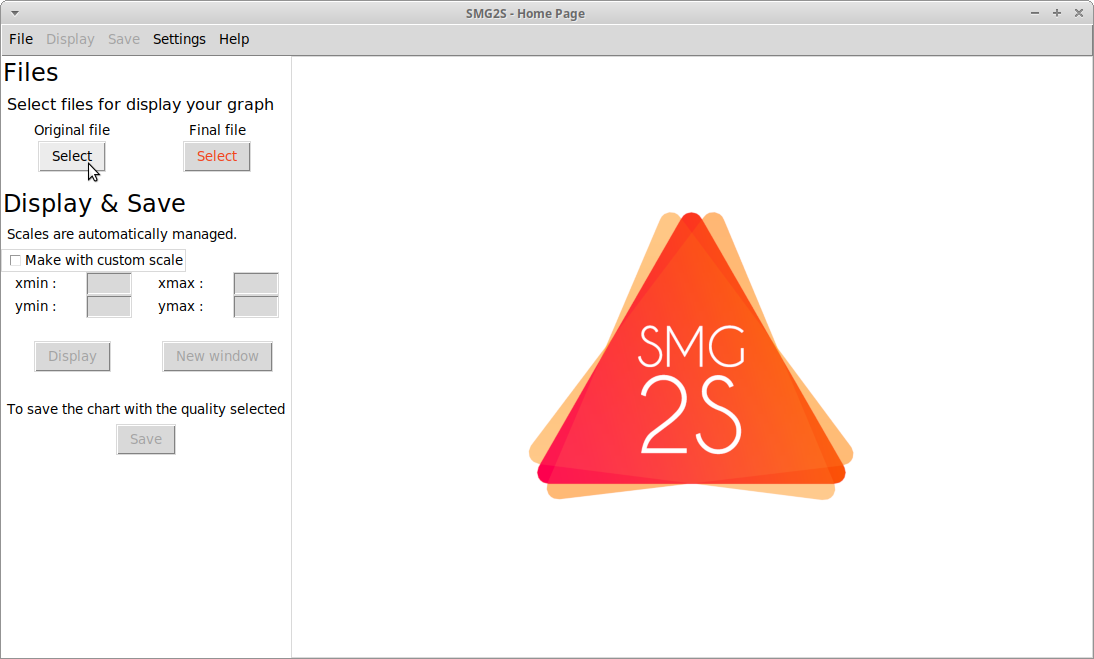
\includegraphics[width=12cm]{home.png}
	\end{figure}

The first step is to select the files which be display. When you have selected a file, the button change in green color as Fig. \ref{fig:Home Screen Capture After selection} (\textcolor{red}{Attention, the files imported should be in the pseudo-Matrix Market vector format} that we have talked):

\begin{figure}[htbp]
			\label{fig:Home Screen Capture After selection}
	\caption{Home Screen Capture After Selection}
		\centering
	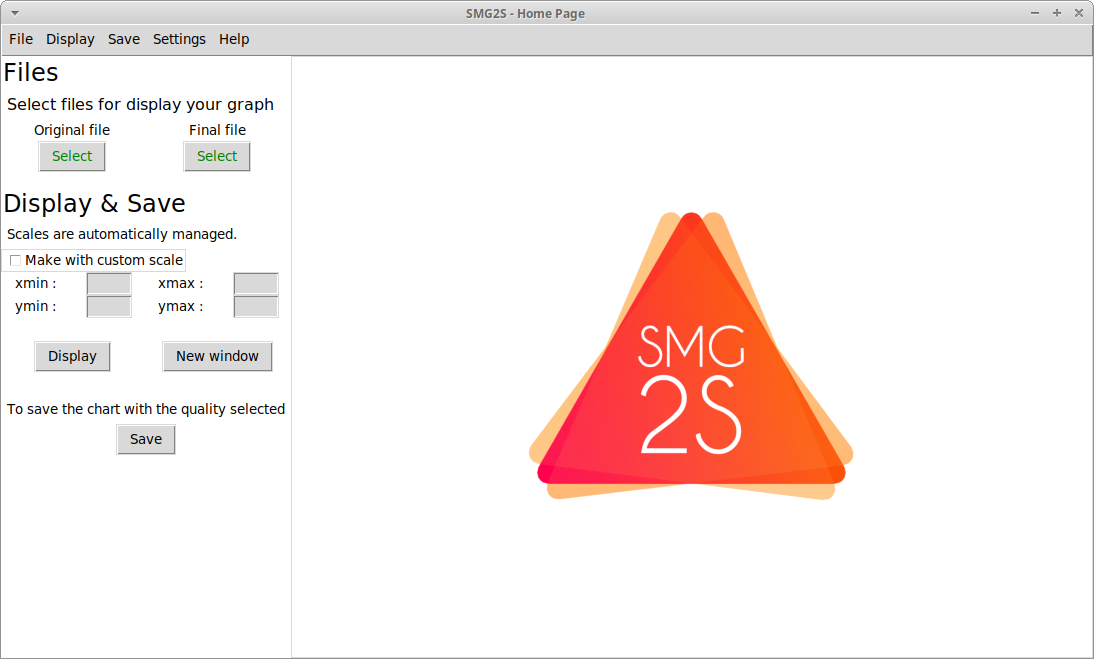
\includegraphics[width=13cm]{home_ready.png}
\end{figure}

After that, you can click on "Display" to build and open the graphic on the right side of the window. Click on "New window" to open your graphic on a new window. It's possible to open as many windows as you want like Fig. \ref{fig:Home Screen Plot Capture}:

\begin{figure}[htbp]
				\label{fig:Home Screen Plot Capture}
	\caption{Home Screen Plot Capture}
		\centering
	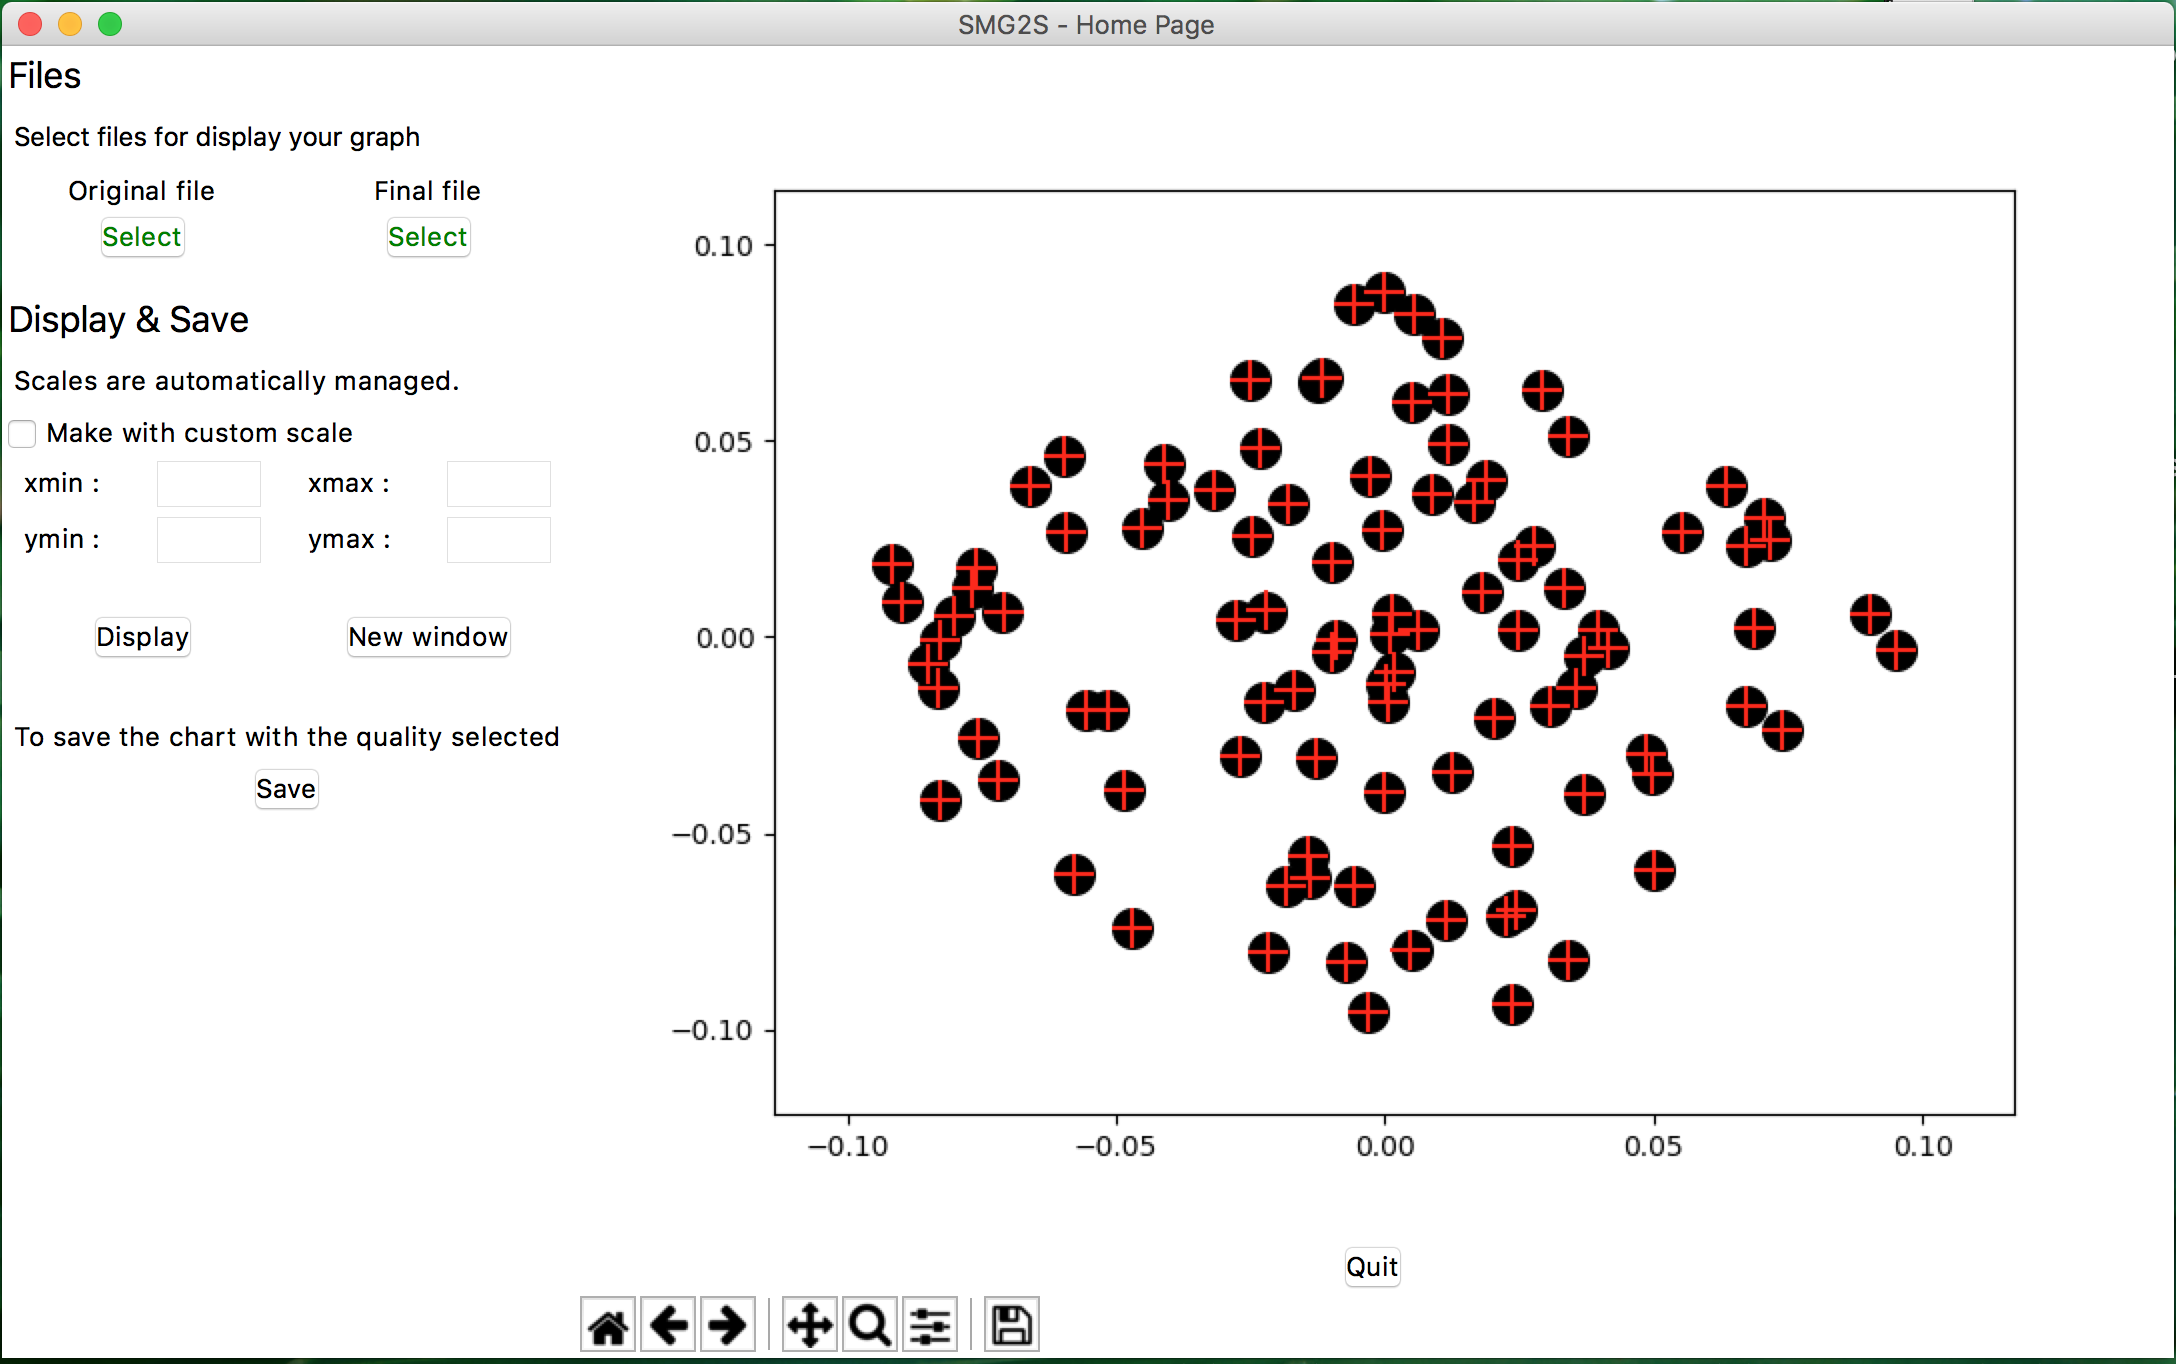
\includegraphics[width=12cm]{home_screen.png}
\end{figure}

Your will be generate with automatic lens scaling, but your can generate it with your own scales as Fig. \ref{fig:Home Screen Plot Capture with lens scaling}:

\begin{figure}[htbp]
	\label{fig:Home Screen Plot Capture with lens scaling}
	\caption{Home Screen Plot Capture with Lens Scaling}
		\centering
	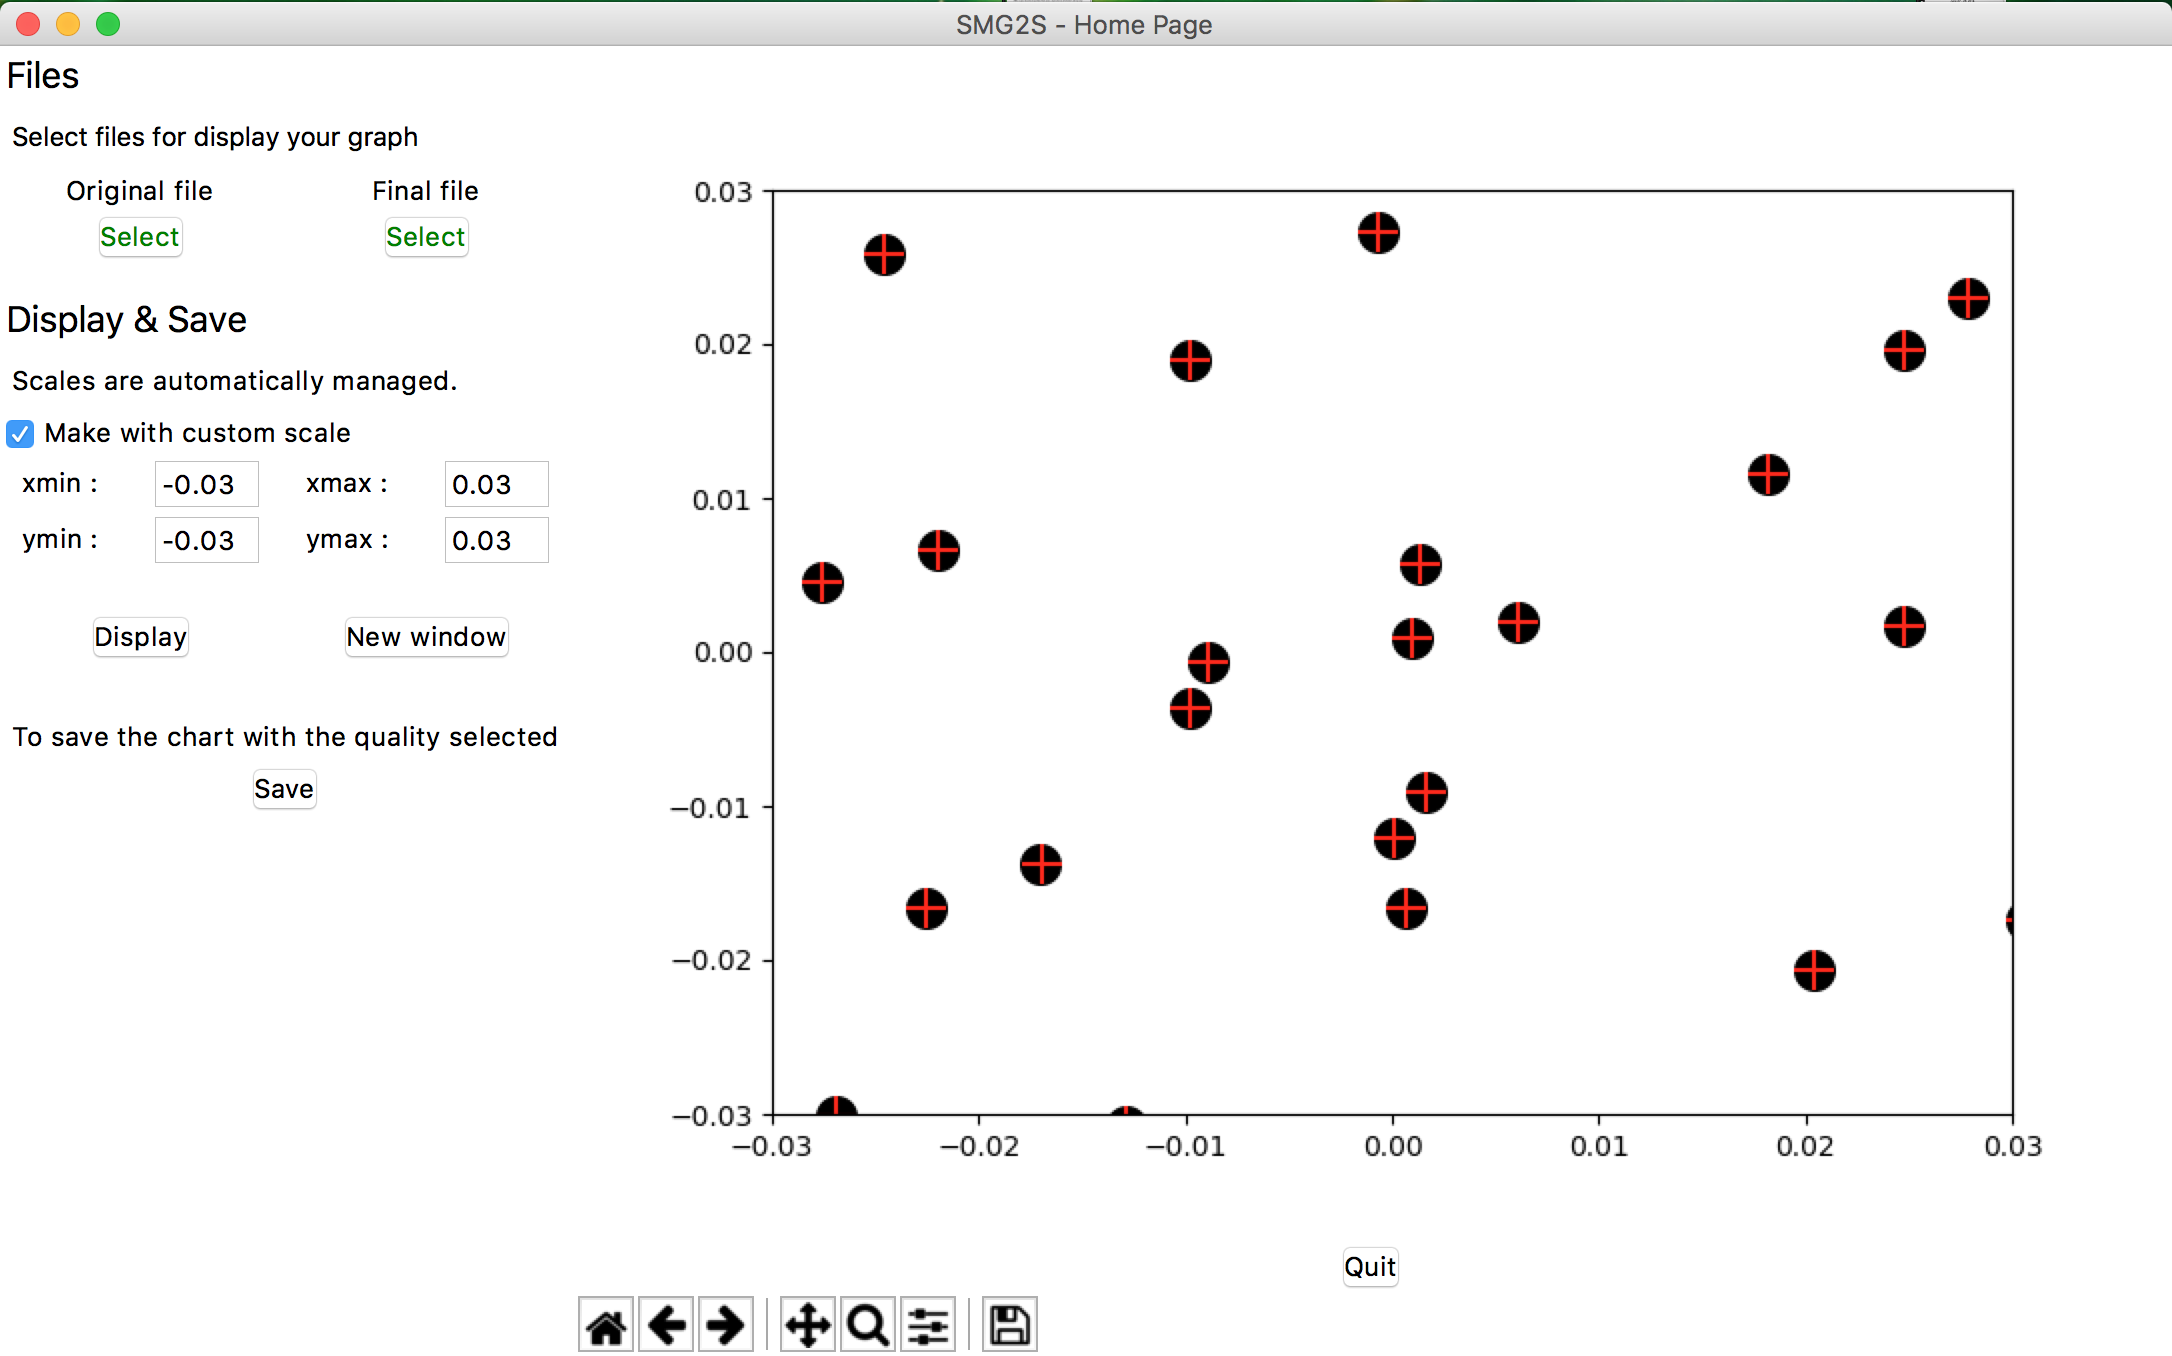
\includegraphics[width=12cm]{home_screen_custom.png}
\end{figure}


	\newpage
	% -------------------------------------------------------------------------------------
	% END DOCUMENT
	% -------------------------------------------------------------------------------------
\end{document}